\section{Method}
\label{section:method}
\subsection{A new empirical gyrochronology relation}

We fit a broken power law to the 650 Myr Praesepe cluster in order to
calibrate a gyrochronology relation that takes advantage of new data available
from the \ktwo\ and \gaia\ surveys.
This relation captures the detailed shape of Praesepe's rotation period-color
relation, and is calibrated to \gaia\ \gcolor\ color.
Praesepe is the ideal calibration cluster because it has the largest number of
members with precisely measured rotation periods, over a large range of colors
\citep[spanning spectral types A0 through M6,][]{rebull2017}, of any open
cluster.
It is relatively tightly clustered on the sky and many of its members were
targeted in a single \ktwo\ campaign, from which rotation periods have been
measured via light curve frequency analysis \citep{douglas2017, rebull2017}.
We compiled rotation periods, \Gaia\ photometry and \gaia\ parallaxes for
members of the 650 Myr Praesepe cluster \citep{fossati2008} by identifying
Praesepe members with measured rotation periods from \citet{douglas2017} in
the \ktwo-\gaia\ crossmatch catalog provided at
\url{https://gaia-kepler.fun/}.
This catalog cross-matched the EPIC catalog \citep{huber2016} with the
Gaia DR2 catalog \citep{brown2018}, using a 1'' search radius.
The result was a sample of 757 stars with rotation periods, parallaxes and
\gaia\ $G$, $G_{BP}$ and $G_{RP}$-band photometry, shown in figure
\ref{fig:praesepe}\footnote{This analysis was performed in a Jupyter notebook
available here: \url{
    https://github.com/RuthAngus/stardate/blob/master/paper/code/Praesepe.ipynb}}.
Although this new model does not perfectly describe the rotation period of
every star, it provides a better representation of rotational evolution than
previous models such as the \citet{angus2015} model (shown as the blue solid
line in figure \ref{fig:praesepe}).
\begin{figure}
  \caption{
    The rotation periods of Praesepe members \citep{douglas2016},
    vs. their \Gaia\ colors (\gcolor) with a broken power law model, fit to
    these data.
    The dashed line and shaded region shows the mean and variance model
    described in equation \ref{eqn:gyro} at 650 Myrs (lower model) and 4.56
    Gyrs (upper model).
    The solid blue line shows the \citep{angus2015} gyrochronology relation at
    650 Myrs (lower model) and 4.56 Gyrs (upper model).
    Shaded regions show the 1$\sigma$ range of the rotation period
    model (equation \ref{eqn:gyro}).
    The rotation periods of stars bluer than around 0.56 dex and redder than
    around 2.7 dex in \gcolor\ are modeled as a broad log-normal distribution
    with a standard deviation of 0.5 dex, added to observational
    uncertainties.
    This figure was generated in a Jupyter notebook available at
    \url{https://github.com/RuthAngus/stardate/blob/master/paper/code/Fitting_Praesepe.ipynb}
}
  \centering
    \includegraphics[width=1.1\textwidth]{Praesepe.pdf}
\label{fig:praesepe}
\end{figure}
In order to fit a relation to Praesepe, we removed rotational outliers bluer
than \gcolor\ = 2.7 via sigma-clipping and fit a 5th-order polynomial to the
remaining FGK and early M stars.
\racomment{We found that a 5th order polynomial provided a substantially
better fit than lower-order polynomials, which were not able to capture the
sharp `elbow’ in the rotation period-color relation. Additional orders
provided either a worse
fit, tending towards extreme values at the boundaries, or diminishing returns
in goodness-of-fit.}
We also fit a straight line to the late M dwarfs (\gcolor\ $>$ 2.7), to
capture the mass-dependent initial rotation periods of low mass stars
\citep{somers2017}.
We fit a separable straight line function to the period-age relation using
the ages of Praesepe and the Sun\footnote{The fitting process was
performed in a Jupyter notebook available at
\url{https://github.com/RuthAngus/stardate/blob/master/paper/code/Fitting_Praesepe.ipynb}.}.
This new Praesepe-calibrated gyrochronology relation is,
\begin{equation}
    \log_{10}(P_\mathrm{rot}) =
    c_A\log_{10}(t) +
    \sum_{n=0}^4 c_n[\log_{10}(G_{BP}-G_{RP})]^n
\label{eqn:fgk_gyro}
\end{equation}
for stars with \gcolor\ $<$ 2.7 and
\begin{equation}
    \log_{10}(P_\mathrm{rot}) =
    c_A\log_{10}(t) +
    \sum_{m=0}^1 b_m[\log_{10}(G_{BP}-G_{RP})]^m
\label{eqn:m_gyro}
\end{equation}
for stars with \gcolor\ $>$ 2.7, where $P_{\mathrm{rot}}$ is rotation period
in days and $t$ is age in years.
Best-fit coefficient values are shown in table \ref{tab:coefficients}.
\begin{table}[h!]
  \begin{center}
      \caption{Coefficient values for equations \ref{eqn:fgk_gyro} and
      \ref{eqn:m_gyro}.}
    \label{tab:coefficients}
    \begin{tabular}{l|c} % <-- Alignments: 1st column left and 2nd middle, with vertical lines in between
      Coefficient & Value  \\
      \hline
      $c_A$ & 0.65 $\pm$ 0.05 \\
      $c_0$ & -4.7 $\pm$ 0.5 \\
      $c_1$ & 0.72 $\pm$ 0.05 \\
      $c_2$ & -4.9 $\pm$ 0.2 \\
      $c_3$ & 29 $\pm$ 2 \\
      $c_4$ & -38 $\pm$ 4 \\
      $b_0$ & 0.9 $\pm$ 0.5 \\
      $b_1$ & -13.6 $\pm$ 0.1 \\
    \end{tabular}
  \end{center}
\end{table}

We calibrated this new relation using Praesepe and the Sun alone, without
including other clusters, because different open clusters have slightly
different period-color relationships \citep{agueros2018, agueros2018b,
curtis2018, curtis2019} and, given that we used an age-color separable
relation, adding in extra clusters was unlikely to improve the calibration.
We did not include asteroseismic stars because most are slightly evolved and
would require a gyrochronology relation that depends on $\log g$.
This new relation, fit to Praesepe and the Sun, does not perfectly predict the
rotation periods of stars at all colors and ages, but it provides several
improvements over previous empirical gyrochronology relations.
Firstly, it uses new \ktwo\ rotation period measurements to model the
period-color relation of Praesepe in detail, secondly, it includes a model for
the rotational behavior of M dwarfs, and thirdly, it is calibrated to \Gaia\
\gcolor\ color: a directly observable quantity and the most widely available
photometric color index.

Equation \ref{eqn:fgk_gyro}, describing the rotational evolution of FGK and
early M stars, is most closely analogous to previously calibrated empirical
gyrochronology relations \citep[\eg][]{barnes2003, barnes2007, mamajek2008,
barnes2010, angus2015}.
It describes stars with Sun-like magnetic dynamos that follow a
`Skumanich-like' magnetic braking law, \ie\ their rotation period increases
with the square root of their age.
It does not describe stars hotter than around 6250 K which have a thin
convective layers and a weak magnetic dynamo, nor does it describe fully
convective stars which take a long time to converge onto the
\citet{skumanich1972} braking law \citep{krishnamurthi1997}.
In addition, stars with Rossby numbers larger than around 2 do not show
Skumanich-like magnetic braking \citep{vansaders2016, vansaders2018}, so
equation \ref{eqn:fgk_gyro} does not describe these stars.
It also does not describe the rotation periods of subgiants or giants, whose
rotation periods are influenced by their expanding radii, changing winds, and
core-to-surface differential rotation \citep[\eg][]{vansaders2013, tayar2018}.
Finally, this relation does not describe the rotation periods of dynamically
or magnetically interacting binaries which often rotate more rapidly than
isolated stars at the same age and color \citep{douglas2016}.
In order to include non-Skumanich type stars in our combined gyrochronal and
isochronal model, we designed a composite gyrochronology relation which
describes a mean and variance model for the rotation period distributions
across the HRD.
Rotation periods are modeled differently for stars of different photometric
color, EEP, Rossby number, age and metallicity.
The rotation period model for each of these groups is described below.
\begin{itemize}
    \item{The rotation periods of late F, GK, and early M dwarfs
        (0.56 $<$ \gcolor\ $<$ 2.7), with Rossby numbers less than 2, are
        modeled as a log-normal distribution, with mean given by equation
        \ref{eqn:fgk_gyro}, and variance given by the squared inverse of their
        observational uncertainties.}
    \item{The rotation periods of fully convective stars (\gcolor\ $>$ 2.7)
        are modeled with a log-normal distribution with mean given by equation
        \ref{eqn:m_gyro}, and an extra standard deviation of
        0.5 dex, added to observational uncertainties.
        This distribution reflects the observed rotation periods of late M
        dwarfs in the Praesepe cluster which span a broad range at every
        color.
        Late M dwarfs with masses $\lesssim$ 0.3 M$_\odot$, temperatures
        $\lesssim$ 3500 and \gcolor $\gtrsim$ 2.7 exhibit weak magnetic
        braking until at least after the age of Praesepe ($\sim$650 million
        years).
    \item{The rotation periods of F-type and hotter stars, with \gcolor\ $<$
        0.56 dex, are modeled as a log-normal distribution with mean,
        $\log_{10}(P_\mathrm{rot})=0.56$,
        and an additional standard deviation, added to observational
        uncertainties, of 0.5 dex.
        Stars more massive than around 1.25 M$_\odot$, with a temperature
        $\gtrsim$ 6250 K and a \gcolor\ $\lesssim$ 0.56 do not spin down
        appreciably over their main-sequence lifetimes because they do not
        have the deep convective envelope needed to generate strong magnetic
        fields.
        This model for the mean and variance of hot star rotation periods is
        based on stars hotter than 6250 K in the \citet{mcquillan2014} sample,
        which have a mean $\log_{10}(P_\mathrm{rot})$ of 0.56 dex and a
        standard deviation of around 0.5 dex.}
        Both hot and cool stars retain rotation periods that are similar to
        their primordial distribution \citep[see \eg][]{matt2012,
        somers2017}.}
    \item{The rotation periods of stars with large Rossby numbers are
        modeled as follows.
        The age at which a star's Rossby number would exceed 2 is calculated
        by inverting equation \ref{eqn:fgk_gyro}.
        If a star's age is greater than this, its mean rotation period is
        given by $P_\mathrm{max} = 2/\tau$, where $\tau$ is the convective
        turnover timescale, calculated via stellar mass using equation 11 from
        \citet{wright2011}.}
    \item{The rotation periods of subgiants are described with a log-normal
        distribution with mean given by equation \ref{eqn:fgk_gyro},
        \ref{eqn:m_gyro} or 0.56, depending on its color, and an additional
        standard deviation of 5 dex.
        This is not an accurate model of subgiant rotation
        periods \citep[see, \eg][]{vansaders2013} but the highly
        inflated variance makes it a weakly constraining one.
        Isochrone fitting provides precise ages for subgiants, so by inflating
        the variance of the gyrochronology relation at large EEP, we allow a
        star's position on the HRD/CMD to dominate the age information over
        its rotation period.
        This is useful because we have not yet built an accurate rotation-age
        relation for subgiants into our model.}
    \item{We model stars younger than around 250 Myrs with a log-normal
        distribution with mean function given by equation \ref{eqn:fgk_gyro},
        \ref{eqn:m_gyro} or 0.56, depending on it whether it has
        an intermediate, red, or blue color respectively and a inflated
        standard deviation of 0.5 dex.
        Rotation periods in young open clusters show a large amount of scatter
        because they have not yet converged onto the \citet{skumanich1972}
        spin-down sequence.}
    \item{Finally, we model stars with very low and high metallicites (-0.2
        $>$ [Fe/H] $>$ 0.2) with a log-normal distribution with mean given by
        equation \ref{eqn:fgk_gyro}, \ref{eqn:m_gyro} or 0.56, depending on
        its color, and a standard deviation of 0.5 dex.
        Gyrochronology is not calibrated at these extreme metallicities due to
        a lack of suitable metal poor and rich calibration stars.
        Rather than assume the same gyrochronology model can be na\"ively
        applied to these stars, we take a more conservative approach and model
        them with a broad Gaussian distribution.}
\end{itemize}
Inflating the variance of the rotation period distribtion for stars with
non-Skumanich magnetic braking behavior has two purposes: 1) in the cases of
hot stars and fully convective stars, it allows the broad distributions of
rotation periods observed in clusters and the field to be matched, and 2) it
down-weights the age-information provided by rotation periods in regions of
the HRD/CMD where rotation periods are not information-rich or the
gyrochronology model is inaccurate or uncalibrated.
If the observational uncertainties on rotation periods are 5\% on average,
which corresponds to 0.05/$\ln(10)$ $\sim$ 0.02 dex, adding 0.5 amounts to
a 25$\times$ increase in standard deviation, or a $\sim$ 600$\times$ increase
in variance.
% The variance on stellar ages inferred via gyrochronology is directly
% proportional to the variance on rotation periods, so a 600$\times$ increase
% in period variance corresponds to a 600$\times$ reduction in the
% age-information provide by gyrochronology, a 600$\times$ increase in
% gyrochronal age variance and a 25$\times$ increase in gyrochronal standard
% deviation.
So, practically speaking, when the standard deviation is inflated to 0.5 dex
or more, ages are almost entirely inferred via isochrone fitting.


We used the following composite gyrochronology model to infer ages from
rotation periods,
\begin{equation}
    \log_{10}(P_\mathrm{rot}) \sim \begin{cases}
        \mathcal{N}\left[(\ref{eqn:fgk_gyro}), (\sigma+\sigma_P)^2\right], & Ro < 2,
        0.56 < G_{BP} - G_{RP} < 2.7 \\
        \mathcal{N}[(\ref{eqn:m_gyro}), (\sigma+\sigma_P)^2], & Ro < 2,
        G_{BP} - G_{RP} > 2.7 \\
        \mathcal{N}[\log_{10}(P_\mathrm{max}), (\sigma+\sigma_P)^2],& Ro \geq 2 \\
        \mathcal{N}[0.56, (\sigma+\sigma_P)^2],& G_{BP} - G_{RP} < 0.56,
    \end{cases}
\label{eqn:gyro}
\end{equation}
where $\sigma$ is the relative period uncertainty, divided by $\ln(10)$, on
individual rotation period measurements and $\sigma_P$ is an additional
scatter that is a function of EEP, age, metallicity and color.
It takes a maximal value of 0.5 for hot stars and fully convective stars, 5
for subgiants and giants, and a minimal value of zero for late F, GK and early
M dwarfs.
The variance model is shown in figure \ref{fig:variance}.
Sigmoid functions were used to provide smooth transitions between regions of
low and high variance.
Sharp changes in variance would produce sharp changes in likelihood, which
would cause the posterior distributions over stellar parameters to be more
difficult to sample.
The sigmoid functions shown in figure \ref{fig:variance} reach half their
maximum values at \gcolor\ = 0.56 and 2.5 for hot and cool stars respectively,
EEP = 454 for subgiants, age = 250 Myrs for young stars, $[$M/H$]$ = -0.2 for
metal poor stars and 0.2 for metal rich stars.
The logistic growth rate, or steepness, of the sigmoid functions is 100
dex$^{-1}$ for both color transitions, .2 EEP$^{-1}$ for the EEP transition,
20 dex$^{-1}$ for the age transition and 5 dex$^{-1}$ for the both metallicity
transitions.
The additional standard deviation is additive, so if a star is \eg\ hot,
evolved and metal poor, the additional standard deviation of its rotation
period rises to 6.

\begin{figure}
  \caption{
    The additional rotation period scatter, $\sigma_P$, added to the
    observational period uncertainties in the model (see equation
    \ref{eqn:gyro}).
    The standard deviation was increased for early F and hotter
    stars (\gcolor $<$ 0.56), late M dwarfs (\gcolor\ $>$ 2.7) and evolved
    stars (EEP $\gtrsim$ 420) in order to down-weight the age-information
    supplied
    by rotation periods and reproduce observed rotation period distributions.
    We also increased the variance for stars younger than around 250 Myrs,
    because the rotation periods of these stars typically have not yet
    converged onto a tight gyrochronology sequence, and for very high and low
    metallicity stars (-0.2 $\gtrsim$ [Fe/H] $\gtrsim$ 0.2) because the
    gyrochronology relations have not been calibrated at these extreme values.
    Down-weighting the gyrochronal likelihood by the inverse variance
    ($1/\sigma^2$) allowed the ages of these stars to be mostly inferred
    via isochrone fitting.
    Sigmoid functions were used to provide smooth transitions between regions
    of low and high variance.
}
  \centering
    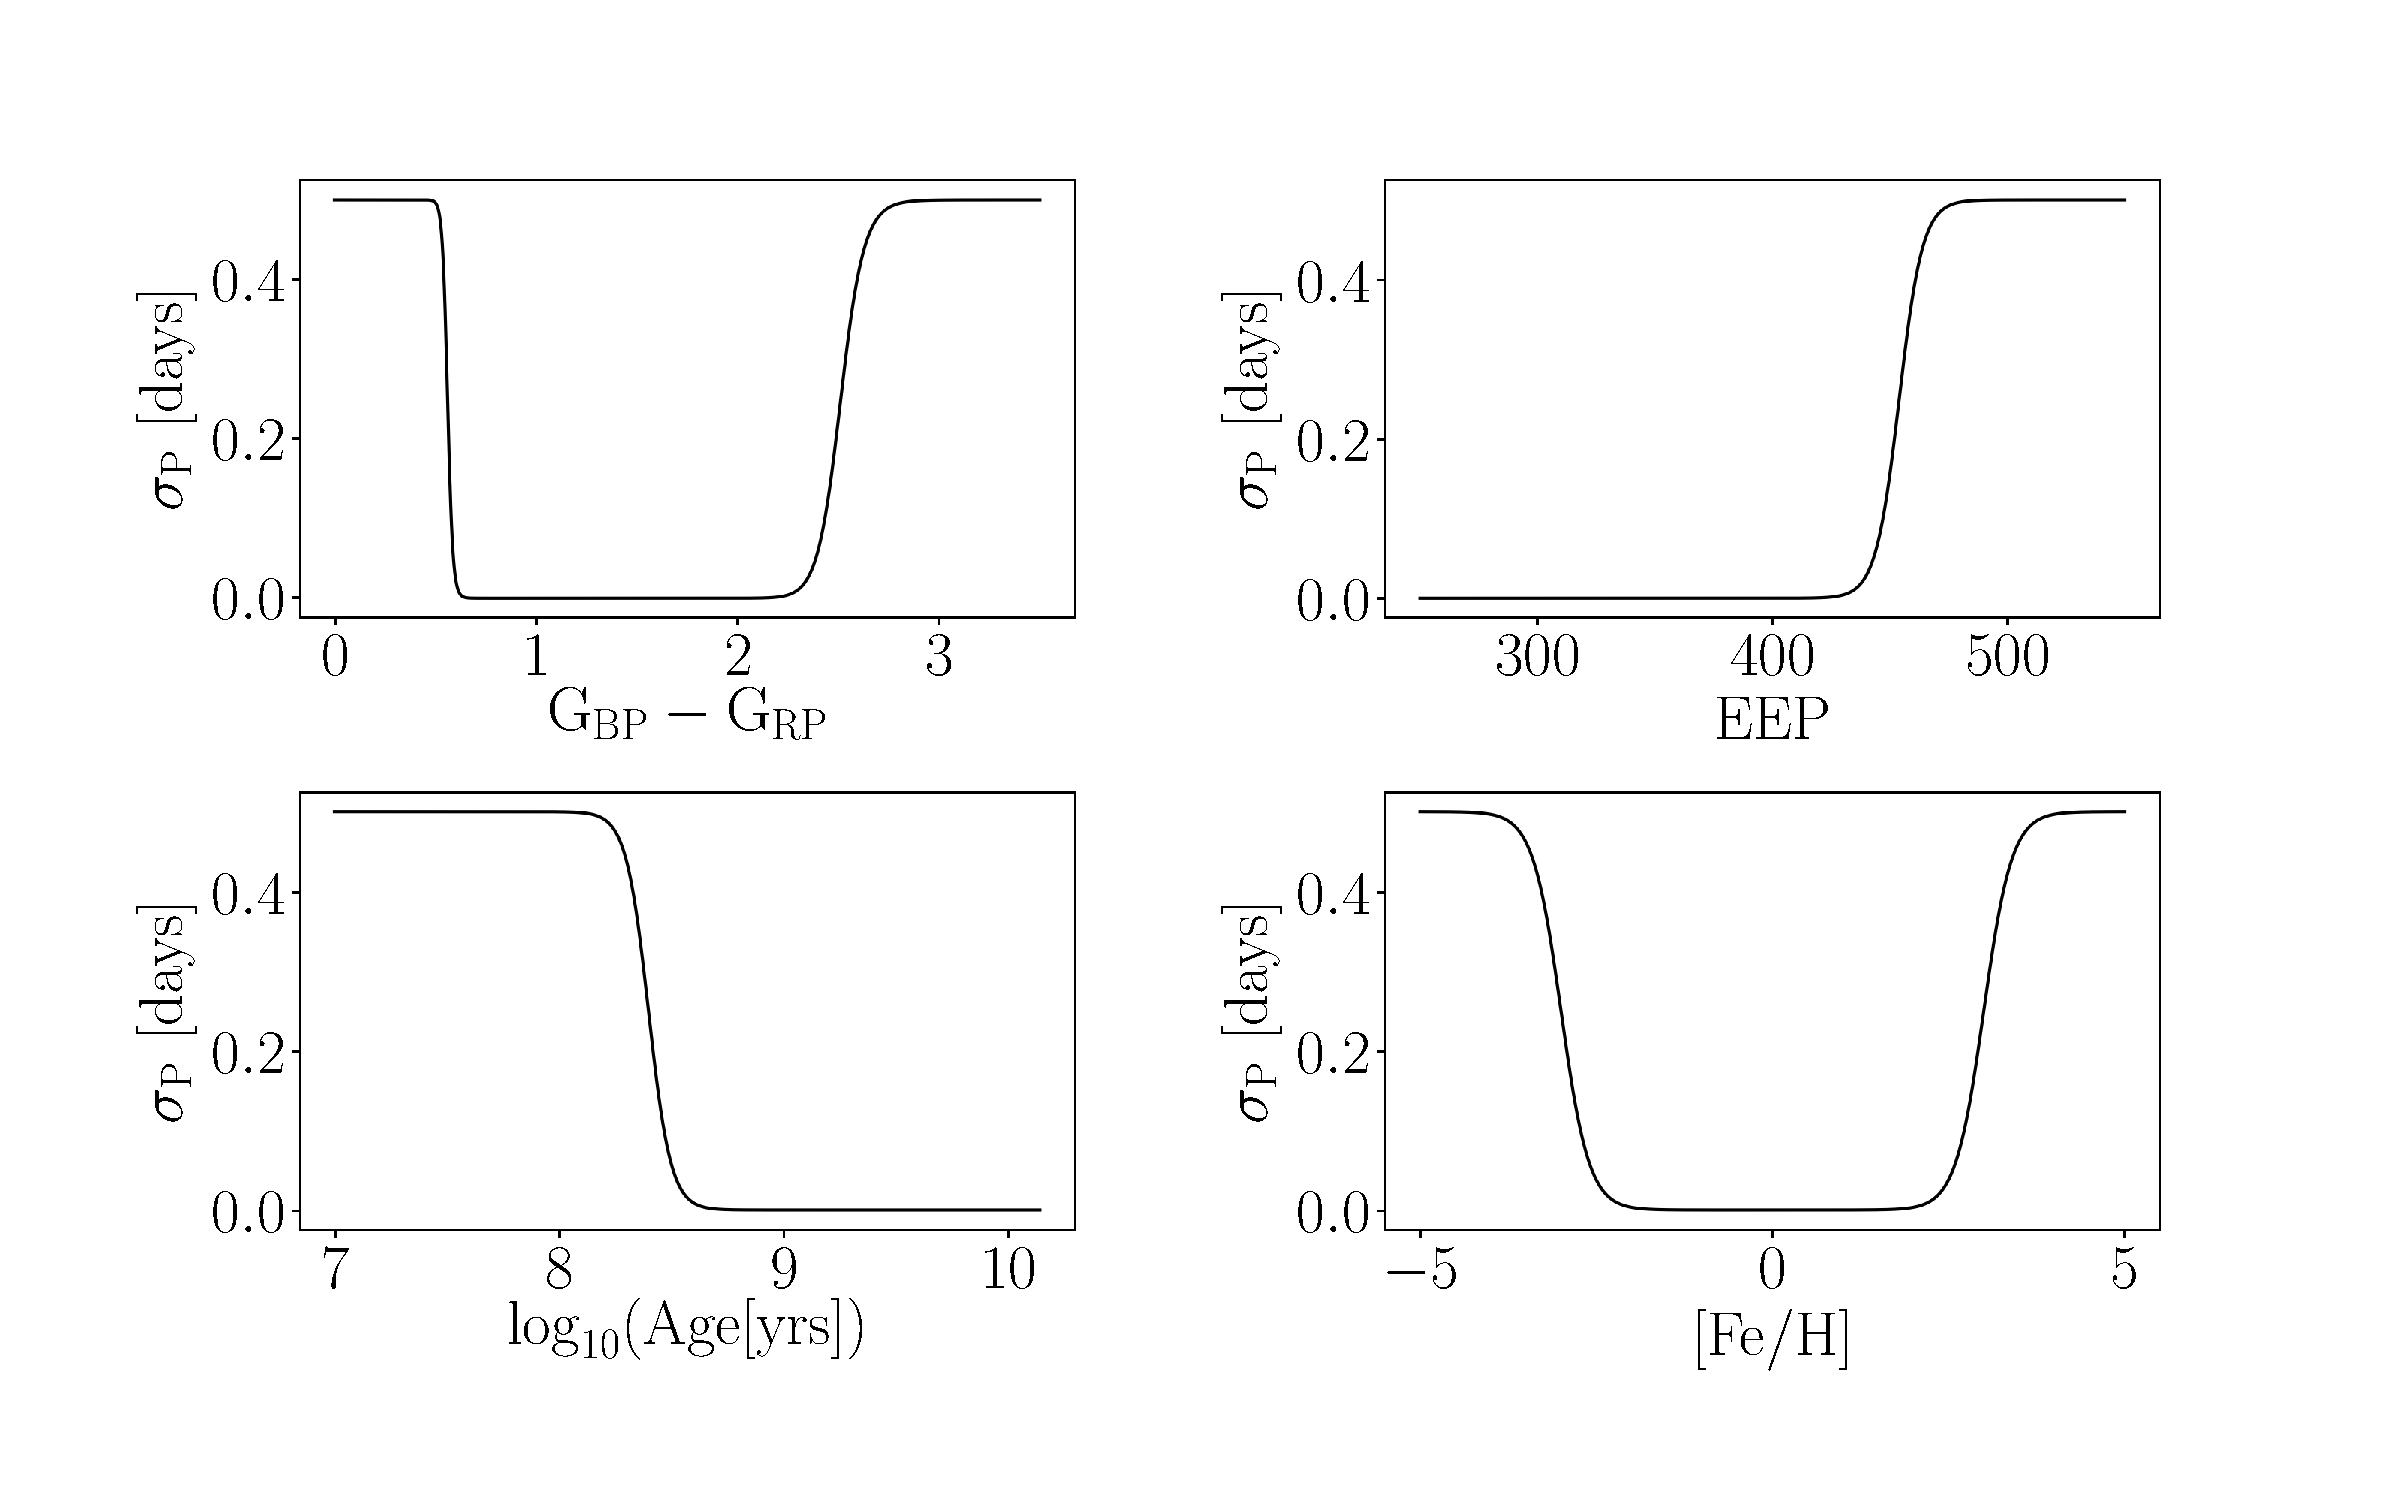
\includegraphics[width=1.\textwidth]{variance}
\label{fig:variance}
\end{figure}

\subsection{Simultaneously fitting gyrochronology and isochrones}
The previous part of this section describes the model for the mean and
variance of rotation periods as a function of their ages (and colors, EEPs,
masses and metallicities).
In what follows, we describe how this model was combined with a stellar
evolution model to infer stellar ages (and other parameters) via
gyrochronology and isochrone fitting simultaneously.
Our goal was to infer the age of a star from its observable properties by
estimating the posterior probability density function (PDF) over age,
\begin{equation} \label{eqn:eqn1}
    % p(t|{\bf m_x}, T_{\mathrm{eff}}, \log(g), \hat{F},
    p(t|{\bf m_x}, P_{\mathrm{rot}}, \bar{\pi}),
\end{equation}
where $t$ is age, ${\bf m_x}$ is a vector of
apparent magnitudes in various bandpasses,
\prot\ is the rotation period and \pmega\ is parallax.
Spectroscopic properties (\teff, \logg\ and $\mathrm{[Fe/H]}$) and/or
asteroseismic parameters (\dnu\ and \numax) may also be available for a star,
in which case they would appear to the right of the `$|$' in the above
equation since they are observables.
In order to calculate a posterior PDF over age, other stellar parameters must
be marginalized over.
These parameters are distance ($D$), V-band extinction ($A_V$), the
inferred metallicity, $[M/H]$\footnote{The inferred metallicity, [M/H] is a
model parameter which is different to the {\it observed} metallicity, [Fe/H]
which would appear on the right side of the $`|'$ in equation \ref{eqn:eqn1}.},
and equivalent evolutionary phase (abbreviated to EEP or
$E$).
EEP is a dimensionless number ranging from around 200 for M dwarfs up
to around 1600 for giants and is 355 for the Sun \citep[see][]{dotter2016,
choi2016}.
Stars are defined as subgiants when their EEP exceeds 454.
Mass is uniquely defined by EEP, age and metallicity.
The marginalization involves integrating over these extra parameters,
\begin{eqnarray} \label{eqn:bayes}
    % & p(A|{\bf m_x}, T_{\mathrm{eff}}, \log(g), \hat{F},
    & p(t|{\bf m_x},
    P_{\mathrm{rot}}, \bar{\pi})
\\ \nonumber
    % & \propto \int p({\bf m_x}, T_{\mathrm{eff}}, \log(g), \hat{F},
    & \propto \int p({\bf m_x},
    P_\mathrm{rot}, \bar{\pi}|
    t, E, [M/H], D, A_V)~p(t)\, p(E)\, p([M/H])\, p(D)\, p(A_V)\, \mathrm{d}E\,
    \mathrm{d}[M/H]\, \mathrm{d}D\, \mathrm{d}A_V.
\end{eqnarray}
This equation is a form of Bayes' rule,
\begin{equation} \label{eqn:eqn2}
\mathrm{Posterior} \propto \mathrm{Likelihood} \times \mathrm{Prior},
\end{equation}
where the likelihood of the data given the model is,
\begin{equation} \label{eqn:full_likelihood}
    % p({\bf m_x}, T_{\mathrm{eff}}, \log(g), \hat{F}, \bar{\pi},
    p({\bf m_x}, \bar{\pi}, P_{\mathrm{rot}}|t, E, D, A_V, [M/H]),
\end{equation}
and the prior PDF over parameters is,
\begin{equation} \label{eqn:prior}
    p(t)\, p(E)\, p(D)\, p(A_V)\, p([M/H]).
\end{equation}
The priors we used are described in the appendix.

We assumed that the process of magnetic braking is independent of hydrogen
burning in the core, outside of the dependencies that are captured in the
model.
This assumption allowed us to multiply two separate likelihood
functions together: one computed using an isochronal model and one computed
using a gyrochronal model.
We assumed that the probability of observing the measured observables given
the model parameters was a Gaussian and that the observables were identically
and independently distributed.
The isochronal likelihood function was,
\begin{eqnarray} \label{eqn:isochrones_only_likelihood}
    % & \mathcal{L_{\mathrm{iso}}} = p({\bf m_x}, T_{\mathrm{eff}}, \log(g),
    & \mathcal{L_{\mathrm{iso}}} = p({\bf m_x},
    \bar{\pi}|t, E, [M/H], D,
    A_V) \\ \nonumber
    & = \frac{1}{\sqrt{(2\pi)^n \det(\Sigma)}}
    \exp\left( -\frac{1}{2} ({\bf O_I} - {\bf I})^T \Sigma ^{-1}
    ({\bf O_I} - {\bf I})\right),
\end{eqnarray}
where ${\bf O_I}$ is the vector of n observables: \pmega, ${\bf m_x}$ plus
spectroscopic and/or asteroseismic observables if available, and $\Sigma$ is
the covariance matrix of that set of observables.
${\bf I}$ is the vector of {\it model} observables that correspond to a set of
parameters: $t$, $E$, $[M/H]$, $D$ and $A_V$, calculated using an isochrone model.
We assumed there is no covariance between these observables and so this
covariance matrix consists of individual parameter variances along the
diagonal with zeros everywhere else.
The gyrochronal likelihood function was,
\begin{eqnarray} \label{eqn:gyro_likelihood}
    & \mathcal{L_{\mathrm{gyro}}} = p(P_\mathrm{rot} |t, E, [M/H], D, A_V) \\ \nonumber
    & = \frac{1}{\sqrt{(2\pi) \det(\Sigma_P)}}
    \exp\left( -\frac{1}{2} ({\bf P_O} - {\bf P_P})^T \Sigma_P ^{-1}
    ({\bf P_O} - {\bf P_P})\right),
\end{eqnarray}
where ${\bf P_O}$ is a 1-D vector of observed logarithmic rotation periods,
and ${\bf P_P}$ is the vector of corresponding logarithmic rotation periods,
predicted by the model.
$\Sigma_P$ was comprised of individual rotation period measurement
uncertainties, plus an additional variance that is a function of EEP and
\gcolor\
color, added in quadrature.
This variance accounts for the stochastic nature of the rotation periods of
very hot and very cool stars and allowed us to predominantly use isochrone
fitting to measure the ages of subgiants.
The full likelihood used in our model was the product of these two likelihood
functions,
\begin{equation}
    \mathcal{L}_{\mathrm{full}} = \mathcal{L}_{\mathrm{iso}} \times
    \mathcal{L}_{\mathrm{gyro}}.
\end{equation}

The inference processes proceded as follows.
First, a set of parameters: age, EEP, metallicity, distance and extinction,
and observables for a single star were passed to the isochronal likelihood
function in equation \eqref{eqn:isochrones_only_likelihood}.
Then, a set of observables corresponding to those parameters were generated
from the MIST model grid using {\tt isochrones.py} \citep{isochrones} and
compared to the measured observables via the isochronal likelihood,
$\mathcal{L}_{\mathrm{iso}}$ (also computed using {\tt isochrones.py}).
The parameters were also passed to the gyrochronology model (equation
\ref{eqn:gyro}) where $t$, $E$,
$[M/H]$, $D$ and $A_V$ were used to calculate \gcolor\ color and mass from the
MIST model grid and, in turn, rotation period via the gyrochronology model.
EEP and \gcolor\ were also used to calculate the additional rotation period
variance, added to the individual period uncertainties.
This model rotation period was compared to the measured rotation period using
gyrochronal likelhood function of equation \ref{eqn:gyro_likelihood}.
The gyrochronal log-likelihood was added to the isochronal log-likelihood to
give the full likelihood, which was then added to the log-prior to produce a
single sample from the posterior PDF.

Ages were inferred with \sd\ using Markov Chain Monte Carlo.
The joint posterior PDF over age, mass, metallicity, distance and extinction
was sampled using the affine invariant ensemble sampler, {\tt emcee}
\citep{foreman-mackey2013} with 24 walkers.
Samples were drawn from the posterior PDF until 100 {\it independent} samples
were obtained.
We actively estimated the autocorrelation length, which indicates how many
steps were taken per independent sample, after every 100 steps using the
autocorrelation tool built into {\tt emcee}.
The MCMC concluded when {\it either} 100 times the autocorrelation length was
reached and the change in autocorrelation length over 100 samples was less
than 0.01, {\it or} the maximum of 500,000 samples was obtained.
This method is trivially parallelizable, since the inference process for each
star can be performed on a separate core.
The age of a single star can be inferred in around 1 hour on a laptop
computer.
